%HEADER
%%%%%%%%%%%%%%%%%%%%%%%%%%%%%%%%%%%%%%%%%%%%%%%%%%%%%%%%%%%%
\documentclass[a4paper, %Format
		11pt, %Font size
		headsepline,
%toc - table of content
		toc=listof, %Include TOC
		toc=listofnumbered, %Number TOC
		toc=bibliography, %Literaturverzeichnis ins TOC
		toc=bibliographynumbered, %Literaturverzeichnis im TOC nummerieren
		]{scrreprt} %Doc class[Optionen]

%Bibliography
%\usepackage{cite} %Paket für Literaturverweise
\usepackage[backend=biber, sorting=none]{biblatex}
\addbibresource{literatur.bib}
%\bibliography{literatur.bib} %Literaturverzeichnis

%GEOMETRIE UND AUSSEHEN
\usepackage[left=35mm,right=30mm,top=15mm,bottom=25mm]{geometry} %Set text geometry
\linespread{1.3}
\setlength{\parindent}{0pt} %disable first line spacing
\usepackage{microtype} %automatically adjust distance between letters

\usepackage{color} %Colorpackage
\definecolor{lightgrey}{rgb}{0.97,0.97,0.97} %definition von "lightgrey"
\usepackage[skip=2pt,font=footnotesize]{caption}


%SONDERZEICHEN UND DEUTSCHE ÜBERSETZUNG
%\usepackage{ucs}<
\usepackage[utf8]{inputenc} %UTF-8 
\usepackage[ngerman, english]{babel}
\usepackage{csquotes}
\usepackage[text]{}
\usepackage{gensymb}

%Tables
\usepackage{booktabs} %extended table options
\usepackage{multirow} %table elements over multiple rows
\usepackage{csvsimple}

%Graphs
\usepackage{graphicx} %Insert graphics
\usepackage{subfig}
\usepackage{xcolor}
\definecolor{titlepagecolor}{cmyk}{1,.60,0,.40}
\definecolor{namecolor}{cmyk}{1,.50,0,.10} 

%Sourcecode
\usepackage{scrhack}
\usepackage{listings} %u.a. Darstellen von Sourcecode
\renewcommand\lstlistingname{Quelltext} %Übersetzung/Umbenennung von "listing" in "Quelltext"
\renewcommand\lstlistlistingname{Quelltextverzeichnis} %Übersetzung von "Quelltextverzeichnis"
%Darstellungsoptionen von Sourcecode
\lstset{numbers=left, numberstyle=\tiny, stepnumber=1, captionpos=b, backgroundcolor=\color{lightgrey}, breaklines=true; float=htbp;} 

%TOC
\usepackage{titletoc}
%\dottedcontents{chapter}[1.5em]{ }{2.3em}{1pc}

%Footnotes
\usepackage{chngcntr}
\counterwithout{footnote}{chapter} %durchgehende, kapitalübergreifende Nummerierung
\setlength{\skip\footins}{10mm} % bestimmt den Abstand zwischen der Grenzlinie der Fußnoten und dem Fließtext.


%Head and Bottom line
\usepackage[singlespacing=true]{scrlayer-scrpage} %Paket für Kopf/Flusszeilen
%\renewcommand*{\chapterpagestyle}{scrheadings} %Seite eines Kapitelbeginn: Linie in Kopfzeile,

%HYPERLINKS
\usepackage{url} %Erleichtert Darstellung von URL (viele Sonderzeichen)
\usepackage[pdftex]{hyperref} %Erstellt Hyperlinks im PDF
% Nach "hyperref" sollten keine weiteren Pakete eingebunden werden,
% da "hyperref" gewisse Befehle umdefiniert.

%%%%%%%%%%%%%%%%%%%%%%%%%%%%%%%%%%%%%%%%%%%%%%%%%%%%%%%%%%%%
%DOKUMENT
\begin{document}

% \clearpairofpagestyles %löscht bisherige Kopf-Fusszeilen Definitionen
% \headsepline{0pt} %Definition der Linienstärke in der Kopfzeile, hier 0

\startcontents[main] % Start TOC

\thispagestyle{empty}
\begin{titlepage}
\center\includegraphics[width=140mm]{Pictures/TitlepageHead}
\vspace*{8mm} %vertikaler Abstand von 10mm
\begin{center} %Text zentriert
	
	\Huge\center\textbf{Hard metrology of the human visual perception}\\ %Große Schrift, Fettschrift
	\vspace*{15mm}
	\Large{by}\\
	\Large{Lukas Schwörer}\\
	\Large{Matriculation number: 65283}\\
	
	\vspace*{11mm}
	
	\Large{A bachelor thesis submitted in partial fulfillment of the}\\
	\Large{requirements for the degree of the}\\
	
	\vspace*{11mm}
	
	\Large{Bachelor of Engineering (B. Eng.)}\\
	\Large{in Mechatronics}\\
	\Large{at Aalen University}\\
	
	\vspace*{11mm}
	
	\Large{Supervisors:}\\
	\Large{Prof. Dr. Ulrich Schmitt (Aalen University)}\\
	\Large{Sabina Rebeggiani (Halmstad University)}\\
	
	\vspace*{11mm}
	
	\Large{Submitted on:}\\
	\Large{November 20\textsuperscript{th}, 2020}\\
\end{center}
\end{titlepage}


%%Leerseite
\thispagestyle{empty}
\hspace{1mm}\\
\newpage

\pagenumbering{roman} %römische Seitenzahlen
\setcounter{page}{1} %Seitenzähler zurücksetzen

\thispagestyle{empty}
\chapter*{Preface}
\addcontentsline{toc}{chapter}{Preface}
\label{preface}

This project is part of the masters degree program "System engineering" of Aalen University and is scheduled to be performed during the first two semesters. This report covers the work realized from April 2021 to February 2022.\\
The practical work and the writing for this project was performed from home.

\vspace*{25mm}

\begin{otherlanguage}{ngerman}
Dieses Projekt ist Teil des Masterstudiengangs "System Engeneering" der Hochschule Aalen und muss während der ersten beiden Semester absolviert werden. Die in diesem Bericht beschriebene praktische Arbeit wurde von Aprill 2021 bis zum Februar 2022 realisiert.\\
Die praktische Arbeit, wie auch das Schreiben des Berichts wurde Zuhause ausgeführt.
\end{otherlanguage} 

\thispagestyle{empty}
\chapter*{Abstract}
\addcontentsline{toc}{chapter}{Abstract}
\label{abstract}

This Project is about the development, setup, testing and qualification of an Electronic Leadscrew (ELS). This project was proposed to the university by myself. 
Its aim is to develop a system to replace the gearbox inside a conventional lathe which will synchronize the rotation of the Leadscrew to the rotation of the spindle.
The ELS needs to be able to keep up with the spindle rotation during conventional turning with different feeds and speeds. In addition to this it should be possible to cut 
precise metric and imperial threads.\\

The electro-mechanical system of the ELS is build around an encoder to read rotational position of the main spindle and a servo motor to control the position of the Leadscrew.
A micro-controller computes the information gathered by the encoder and commands the servo-motor to the correct positions.\\

To be able to easily change and add Features as well as to predict the behavior of the system the development of the ELS needs to be model based. This model needs to incorporate all aspects
of the system including the spindle, the encoder, the micro-controller and the servo motor. As comparison the conventional gearbox should also be modeled.\\



\thispagestyle{empty}
\chapter*{Kurzfassung}
\addcontentsline{toc}{chapter}{Kurzfassung}
\label{kurzfassung}
\begin{otherlanguage}{ngerman}

    Dieses Projekt beschäftigt sich mit der Entwicklung, dem Aufbau, dem Testen und Qualifizieren einer Elektronischen Leitspindel (ELS). Dieses Projekt wurde der Universität von mir vorgeschlagen, da es aufgrund der Covid-19 Pandemie nur begrenzt möglich war praktische Projekte durchzuführen. Sein Ziel ist es ein System zu entwickeln, dass das Getriebe in einer konventionellen Drehbank ersetzt und die Rotation der Leitspindel zu der Rotation der Hauptspindel synchronisiert. Die ELS muss fähig sein, mit der Rotation der Hauptspindel mitzuhalten während einer konventionellen Drehbearbeitung mit unterschiedlichen Drehzahlen und Vorschüben. Zusätzlich muss es möglich sein, präzise metrische und imperische Gewinde herzustellen.\\
 
    Das elektromechanische System der ELS besteht aus einem Encoder, der die Position der Hauptspindel ausliest und einem Servomotor, der die Position der Leitspindel kontrolliert. Ein Mikrocontroller
    verarbeitet die vom Encoder gesammelten Informationen und bestimmt die korrekte Position des Servomotors.\\
    Um ein einfaches Ändern und Entfernen von Features zu ermöglichen und das Verhalten des Systems vorherzusagen, muss die Entwicklung der ELS Modellbasiert durchgeführt werden. Dieses Modell muss alle Komponenten des reellen Systems beinhalten, eingeschlossen der Spindel, des Encoders, dem Mikrocontroller und dem Servomotor. Zum Vergleich sollte auch ein System mit einem konventionellen Getriebe modelliert werden.
    
\end{otherlanguage}


\thispagestyle{empty}
\chapter*{Acknowledgement}
\addcontentsline{toc}{chapter}{Acknowledgement}
\label{acknowledgement}
At this point I would like to thank the following people who made this project possible:

\begin{itemize}
    \item \textbf{Prof. Dr. Markus Glaser} For supervising and supporting my project.
    \item \textbf{James Clough (Clough42)} For helping me to find hardware matching my specifications and supplying me with the great documentation about his own ELS project. 
\end{itemize}


% Insert TOC
\renewcommand\contentsname{\huge Table of Contents}% Change TOC Name and size
\printcontents[main]{ }{0}{\section*{\contentsname}}
\newpage

%KOPF-/FUSSZEILE
\pagestyle{scrheadings} 
% \clearpairofpagestyles %löscht bisherige Kopf-Fusszeilen Definitionen
% \automark[]{chapter} %[rechte Seite]{linke Seite}
% \chead[]{\headmark} %oben mitte
% \cfoot[\pagemark]{\pagemark} %Seitenzahlen auf [Seite des Kapitelbeginns]{den folgenden Seiten}
% \headsepline{0.5pt} %Definition der Linienstärke in der Kopfzeile, hier 0,5

\newpage
\pagenumbering{arabic} %arabische Seitenzahlen
\setcounter{page}{1} %Seitenzähler zurücksetzen

\chapter{Introduction}
\label{introductio}

This chapter will highlight the working environment, the project background as well as its aim.
 
\section{Working environment}
 
\subsection{University of Aalen}
The university of Aalen was founded in 1962 and by now is one of the leading university's of applied sciences in Germany. It has a focus in technical and economic research and has approximately 6000 students.
The University is located in Aalen, a smaller city in the south of Germany. The University has ongoing cooperations with many companies in the region such as Zeiss, Mapal and Trumpf. Further, Aalen University has international cooperations with 136 other Universities.\cite{Aalen}
 
\subsection{Workshop}
The practical part of this project was carried out in my home workshop. The workshop has tools for basic metal work, wood work, a 3D-Printing as well as some tools for the development of electronics. Further, equipment for welding, conventional milling and turning is available.
 
 
\section{Project background}
The mechatronic project is fixed part of the masters program "System Engineering" at Aalen University. It is supposed to cover both practical and theoretical work for solving a mechatronic problem.\\
In the theoretical part of the project, the problem needs to be split in smaller individual issues. In the next step, solutions for each of the issues need to be found by thoroughly analyzing the requirements of the projects.\\
In the practical part of the project, the previously discovered issues and the solutions for it are supposed to be translated and tested to their functionality in practice.\\
This development process can be summarized in the so called V-Modell. The V-Modell is shown in \ref{V-Model Complete}.
 
\begin{figure}
    \begin{center}
    \includegraphics[width=12cm]{Pictures/VModelComplete.png}
    \caption[V-Model Complete]{V-Model}
    \label{V-Model Complete}
    \end{center}
\end{figure}
 
The motivation and idea of this project were founded by my interest in metal work as well as online sources about similar projects.\cite{CloughELS}
 
\subsection{Aim of study}
The aim of this project is to add the Electronic Lead screw system to the Emco Compact 8 mini Lathe (see Appendix \ref{AppendixListOfCompanies}) in a way that is reversible. This is important in order to remain the value of the lathe. Further, the ELS system is supposed to be an addition that speeds up and simplifies the manual operation of the lathe by replacing the manual gearbox with electronics. For this reason, it is not planned to add servos to the other axis of the lathe in the future. Both, the Lathe as well as the Gearbox that is going to be replaced are shown in Figure \ref{AimLathe}.
 
 

\begin{figure}
    \begin{center}
    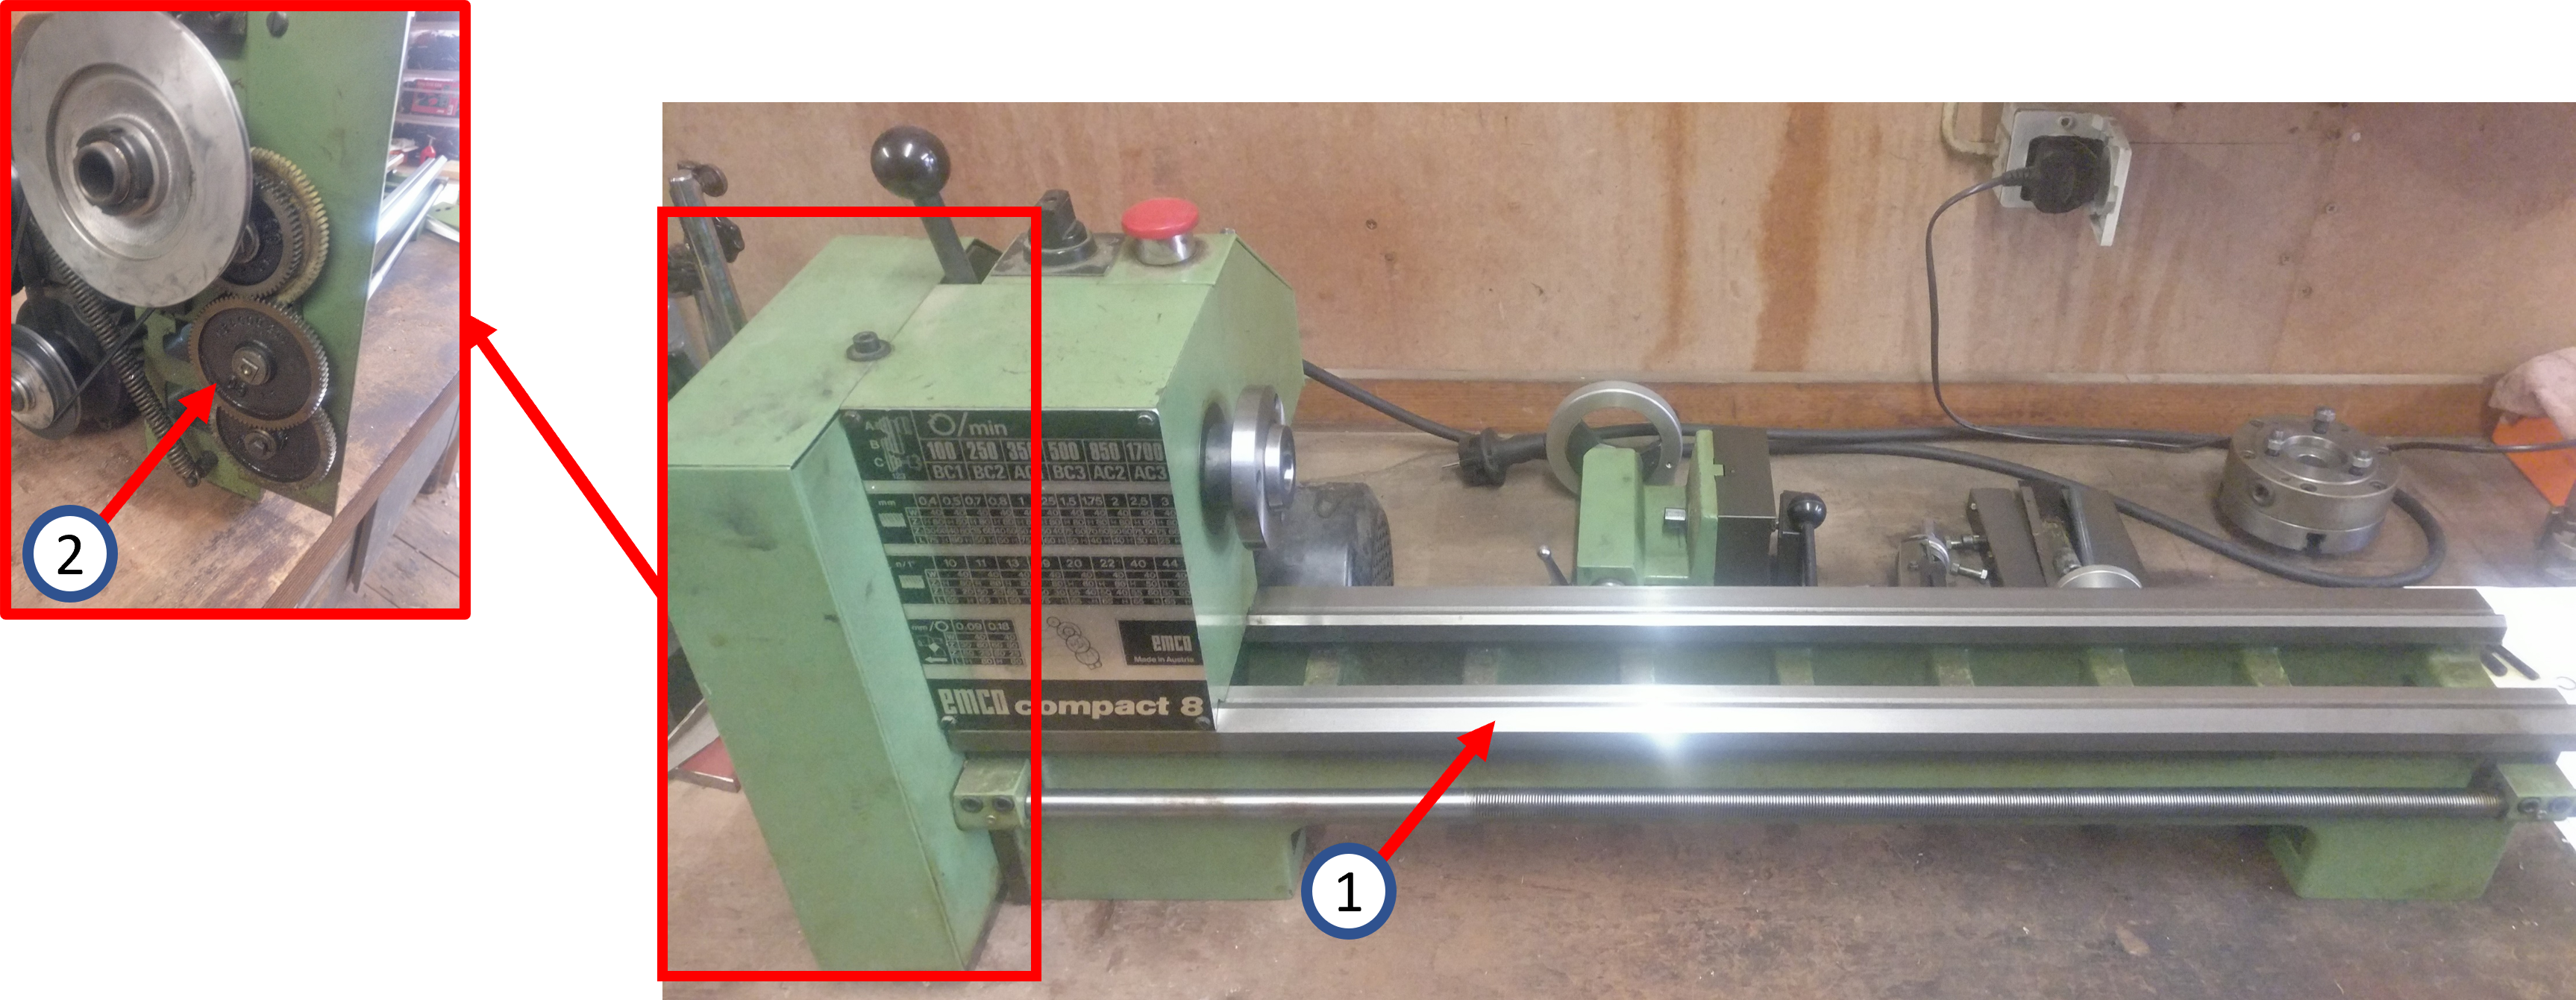
\includegraphics[width=12cm]{Pictures/AimLathe.png}
    \caption[Image of the Emco Compact 8 and the manual gearbox]{Image of the Emco Compact 8 and the manual gearbox; 1 - Emco Compact 8, 2 - Manual gearbox}
    \label{AimLathe}
    \end{center}
\end{figure}





\chapter{Theoretical Background}
\label{theoretical_background}

\section{Numerical Mathmatic}
\subsection{Fractional Mathmatic}
\subsection{Floatingpoint Mathmatic}

\section{Motors}

\section{Manufactoring}
\subsection{Additive Manufactoring}
\subsection{Subtractive Manufactoring}


\chapter{Hardware and Software}
\label{hardwareandsoftware}

\section{Hardware}

\section{Software}
\subsection{Matlab - Simulink}
\subsection{Code Composer Studio}
\subsection{Python}
\subsection{Git}


\chapter{Experimental}
\label{experimental}
\section{Model in the Loop}
\subsection{Initial Considerations}
\subsection{Parameter Identification}
\subsection{Simulink Model}
\subsubsection{Encoder and Spindel}
\subsubsection{Microcontroler}
\subsubsection{Stepper Motor}
\subsubsection{Gearbox}
\subsection{Code Generation}
\subsection{Mechanical Implementation}

\section{Software in the Loop}
\subsection{Logic}
\subsection{Arithmetic}

\section{Hardware in the Loop}
\subsection{Component Test}
\subsection{System Test}
\subsection{Integration Test}
\subsubsection{Turning}
\subsubsection{Threading}











\chapter{Results and Discussion}
\label{resultanddiscussion}
\begin{figure}[h!]
    \begin{center}
    \includegraphics[width=12cm]{Pictures/V Model Qualification.png}
    \caption[V Model Qualification]{V Model Qualification Stage}
    \label{V Model Qualification}
    \end{center}
\end{figure}
\subsection{Arythmatic}
\subsection{Threading}
\subsection{Turning}

\chapter{Outlook}
\label{outlook}
The Electronic Lead screw system offers due to the modularity of the control software and the interface the opportunity to add further functions to the system. In the future, modes for circular grinding as well as partially automated threading are planned. However, more important additions to the Electronic Lead screw system will be a cabinet for the electronics. This cabinet and its components were already planned and ordered during the project, but did not arrive in time due to a global electronics shortage.\\
Further, a Variable Speed Drive (VSD) will be added to the main spindle in the future. A VSD enables the operator to control the speed of the main spindle step-less. In addition to that, the VSD could be controlled connected to the ELS. This would enable features such as automatic threading or turning.




\listoffigures %Abbildungsverzeichnis

\listoftables %Tabellenverzeichnis

%\lstlistoflistings %Quelltextverzeichnis

%\printnomenclature %Abkürzungsverzeichnis

\renewcommand{\bibname}{References}
\printbibliography


%ANHANG
\cleardoublepage
\pagenumbering{Roman} %Big romanian Pagenumbering
\setcounter{page}{1} %Seitenzähler zurücksetzen

\thispagestyle{plain}
\appendix %Anhang einfügen


%TABLE OF CONTENTS APPENDIX
\phantomsection
\addcontentsline{toc}{chapter}{Appendix}
\startcontents[appendix]
\renewcommand\contentsname{\huge Appendix}% if a change of the default "Contents" name is required
\printcontents[appendix]{ }{0}{\section*{\contentsname}}
\stopcontents[main]
\newpage
%APPENDIX

\thispagestyle{empty}
\chapter{Additional Topics}
\label{AppendixAdditionalTopics}

\section{Pin Out}

\section{External Reset}

% \begin{figure}[h!]
% \begin{center}
% \includegraphics[width=12cm]{Pictures/}
% \caption[VERZEICHNISEINTRAG]{BESCHRIFTUNG}
% \label{OpticalTableCompliance}
% \end{center}
% \end{figure}


\thispagestyle{empty}
\chapter{List of Companies}
\label{AppendixListOfCompanies}

\begin{figure}[h!]
\includegraphics[height=1.6cm]{Pictures/EmcoLogo.png}
\end{figure}
\vspace{3mm}
Company:  EMCO GmbH\\
Website: \url{https://www.emco-world.com/}
\vspace{5mm}
\hrule
\vspace{10mm}

\begin{figure}[h!]
\includegraphics[height=1.6cm]{Pictures/KivyLogo.jpg}
\end{figure}
\vspace{3mm}
Company: Kivy.org\\
Website: \url{https://kivy.org/}
\vspace{5mm}
\hrule
\vspace{10mm}

\begin{figure}[h!]
\includegraphics[height=1.6cm]{Pictures/AppMathworksLogo}
\end{figure}
\vspace{3mm}
Company: The MathWorks, Inc.\\
Website: \url{https://www.mathworks.com/}
\vspace{5mm}
\hrule
\vspace{10mm}

\begin{figure}[h!]
\includegraphics[height=1.6cm]{Pictures/OpkonLogo.jpg}
\end{figure}
\vspace{3mm}
Company: OPKON Optic Electronic A.Ş.\\
Website: \url{https://www.opkon.com.tr/}
\vspace{5mm}
\hrule
\vspace{10mm}

\begin{figure}[h!]
\includegraphics[height=1.6cm]{Pictures/Raspberry_Pi_Logo.jpg}
\end{figure}
\vspace{3mm}
Company:  Raspberry Pi Foundation\\
Website: \url{https://www.raspberrypi.org/}
\vspace{5mm}
\hrule
\vspace{10mm}

\begin{figure}[h!]
\includegraphics[height=1.6cm]{Pictures/StepperonlineLogo.jpg}
\end{figure}
\vspace{3mm}
Company:  STEPPERONLINE, Inc.\\
Website: \url{https://www.omc-stepperonline.com/}
\vspace{5mm}
\hrule
\vspace{10mm}

\begin{figure}[h!]
\includegraphics[height=1.6cm]{Pictures/TexasInstruments-Logo.png}
\end{figure}
\vspace{3mm}
Company: Texas Instruments, Inc.\\
Website: \url{https://www.ti.com/}
\vspace{5mm}
\hrule
\vspace{10mm}



\thispagestyle{empty}
\chapter{Requirements ELS}
\label{AppendixRequirements}
\begin{figure}[!h]
    \includegraphics[width=12cm]{Pictures/AppRequ1.png}
    \caption[System requirements table 1]{System requirements table 1}
\end{figure}

\begin{figure}[!h]
    \includegraphics[width=12cm]{Pictures/AppRequ2.png}
    \caption[System requirements table 2]{System requirements table 2}
\end{figure}

\thispagestyle{empty}
\chapter{Organisation Chart}
\label{AppChart}

\thispagestyle{empty}
\chapter{Source Code}
\label{appendixSoureCode}

\newpage
\section{main.c}
\lstloadlanguages{C}%
\lstinputlisting[language = C, 
		firstline = 1, %Beginn bei Zeile XX aus Datei
		firstnumber = 1] %Beginn der Nummerierung 
		{../CSS/main.c} %{einzulesende Datei}

% \newpage
% \section{Configuration.h}
% \lstloadlanguages{C}%
% \lstinputlisting[language = C, 
% 		firstline = 1, %Beginn bei Zeile XX aus Datei
% 		firstnumber = 1] %Beginn der Nummerierung 
% 		{../CSS/Configuration.h} %{einzulesende Datei}

% \newpage
% \section{Configuration.c}
% \lstloadlanguages{C}%
% \lstinputlisting[language = C, 
% 		firstline = 1, %Beginn bei Zeile XX aus Datei
% 		firstnumber = 1] %Beginn der Nummerierung 
% 		{../CSS/Configuration.c} %{einzulesende Datei}

\newpage
\section{MainUI.py}
\lstloadlanguages{Python}%
\lstinputlisting[language = Python, 
		firstline = 1, %Beginn bei Zeile XX aus Datei
		firstnumber = 1] %Beginn der Nummerierung 
		{../Python/MainUI.py} %{einzulesende Datei}

\stopcontents[appendix]

%\begin{otherlanguage}{ngerman}
\addchap*{Eidesstattliche Erklärung}

\vspace*{5mm}

\thispagestyle{empty}

\begin{flushleft}
\begin{tabular}[h]{p{60mm}l p{60mm}l}
\textbf{Name:} Schwörer 			&\textbf{Vorname:} Lukas\\
\textbf{Matrikel-Nr.:} 65283		&\textbf{Studiengang:} Mechatronik\\
\end{tabular}
\end{flushleft}

\vspace*{11mm}

Hiermit versichere ich, \textbf{Lukas Schwörer}, an Eides statt, dass ich die vorliegende Bachelorarbeit

an der \textbf{University of Halmstad}

mit dem Titel \textbf{„Hard metrology of the human visual perception“}

selbständig und ohne fremde Hilfe verfasst und keine anderen als die angegebenen Hilfsmittel benutzt habe. Die Stellen der Arbeit, die dem Wortlaut oder dem Sinne nach anderen Werken entnommen wurden, sind in jedem Fall unter Angabe der Quelle kenntlich gemacht.\\

Ich habe die Bedeutung der eidesstattlichen Versicherung und prüfungsrechtlichen Folgen (\S 23 Abs. 3 des allg. Teils der Bachelor-SPO der Hochschule Aalen) sowie die strafrechtlichen Folgen (siehe unten) einer unrichtigen oder unvollständigen eidesstattlichen Versicherung zur Kenntnis genommen.\\

\vspace*{10mm}
\Large\textbf{Auszug aus dem Strafgesetzbuch (StGB)}


\normalsize\textbf{\S 156 StGB} Falsche Versicherung an Eides Statt
Wer von einer zur Abnahme einer Versicherung an Eides Statt zuständigen Behörde eine solche Versicherung falsch abgibt oder unter Berufung auf eine solche Versicherung falsch aussagt, wird mit Freiheitsstrafe bis zu drei Jahren oder mit Geldstrafe bestraft.

\vspace*{25mm}


\rule[-0.2cm]{5cm}{0.5pt} \hspace*{30mm}\rule[-0.2cm]{5cm}{0.5pt}
\newline
Ort, Datum\hspace*{61.85mm}Unterschrift

\end{otherlanguage} 


\end{document}
%%%%%%%%%%%%%%%%%%%%%%%%%%%%%%%%%%%%%%%%%%%%%%%%%%%%%%%%%%%%
%END_OF_FILE















